\documentclass{article}
\usepackage{iclr2027_conference,times}
% \iclrfinalcopy is deliberately NOT declared: the style then renders
% "Anonymous authors / Paper under double-blind review". Declaring it would
% de-anonymise the submission and trigger desk rejection.
%
% Line-number rulers suppressed at the author's request. This keeps anonymous
% mode intact -- we blank the ruler macro rather than setting \iclrfinalcopy,
% which would have revealed identity.
\makeatletter
\def\iclrruler#1{}
\makeatother

\usepackage{amsmath,amssymb,amsfonts,amsthm}
\usepackage{graphicx}
\usepackage{xcolor}
\usepackage{colortbl}
\usepackage{booktabs}
\usepackage{multirow}
\usepackage{array}
\usepackage{tikz}
\usepackage{pgfplots}
\pgfplotsset{compat=1.17}
\usetikzlibrary{arrows.meta,patterns,decorations.pathreplacing,positioning}
\usepackage{hyperref}
\usepackage{url}
\usepackage{microtype}

\theoremstyle{definition}\newtheorem{remark}{Remark}
\theoremstyle{plain}\newtheorem{proposition}{Proposition}

\definecolor{hl}{RGB}{232,238,250}
\definecolor{bad}{RGB}{168,62,42}
\definecolor{keep}{RGB}{38,70,142}
\definecolor{keepL}{RGB}{200,214,240}
\definecolor{lose}{RGB}{176,58,46}
\definecolor{loseL}{RGB}{244,214,208}
\definecolor{fade1}{RGB}{88,112,180}
\definecolor{fade2}{RGB}{140,158,205}
\definecolor{fade3}{RGB}{190,200,225}
\definecolor{neut}{RGB}{120,120,124}

\title{Demotion Beats Deletion: Graded Forgetting for\\Capacity-Bounded Agent Memory}

% Anonymised for double-blind review.
\author{Anonymous}

\begin{document}
\maketitle

\begin{abstract}
Persistent LLM agents accumulate memory faster than they can afford to read it,
and every deployed system resolves this by deleting. Anthropic's Memory Stores
cap a store at 10{,}000 entries and instruct operators to remove stale ones;
Mem0 prunes through LLM-issued \texttt{DELETE}; ChatGPT's background
consolidation rewrites in place. Deletion is an irreversible decision taken
without knowing which memory a future query will need. We ask whether it is
necessary. We present \textbf{graded forgetting}: traces are demoted through
discrete retention stages and compressed to progressively lossier fidelity
tiers, but never removed, so a capacity budget is met by shedding \emph{detail}
rather than \emph{items}. We introduce \textbf{recall-after-eviction}, a
protocol that isolates the capability at stake by conditioning on questions
whose supporting evidence a capacity bound has destroyed. On an 833-day,
1{,}115-memory timeline held to 35\% of its full size, deletion answers
\textbf{2.5\%} of questions about the evicted past while graded forgetting
answers \textbf{60.0\%} - 80\% of the uncapped ceiling, from the same byte
budget. We report equally clearly that graded forgetting does \emph{not} improve
ordinary retrieval: across six settings, two backbones, a production memory
platform and a third-party baseline, it is never better and usually worse. The
contribution is therefore a capability under capacity pressure, not an accuracy
gain, and we argue this is the axis on which agent memory should be evaluated.
\end{abstract}

% =====================================================================
\section{Introduction}

Managed agent memory is deployed infrastructure. Anthropic's Memory Stores
\citep{anthropic2026memory} mount a persistent, versioned document collection
into an agent's sandbox. Mem0 \citep{chhikara2025mem0} maintains a compact fact
store through LLM-driven add/update/delete. OpenAI's ChatGPT synthesises
long-horizon user memory in a background pass \citep{openai2026dreaming}. The
question is no longer whether an agent can remember, but what it should stop
remembering.

Every one of these answers by deletion, and their own documentation is explicit
about the consequence:

\begin{quote}\small
``When a store reaches its \textbf{10,000-memory limit}, writes to new memories
fail\ldots{} \textbf{Delete stale or redundant memories}\ldots{} Switch your
sessions over to that output store, then archive or delete the
original.'' \citep{anthropic2026memory}
\end{quote}

Deletion is irreversible and is decided without knowledge of future queries. A
memory judged stale today is unavailable tomorrow at any cue strength. This is
the failure mode we target.

\paragraph{Graded forgetting.} Human memory does not delete; it fades, and
faded traces return under sufficient contextual support
\citep{proust1913,aggleton1999,tulving1983}. We operationalise this as a
lifecycle over an ordinary memory store: each trace carries a retention stage
$k$ that advances with disuse and a fidelity tier $\ell$ that rises with $k$,
discarding episodic detail while retaining a routing scaffold. A capacity
budget is met by \emph{compressing} rather than \emph{removing}, so every trace
remains addressable, in degraded form, indefinitely.

\paragraph{What we measure, and what we found.} Our headline result is narrow
and, we believe, the right shape for this problem. Under a hard capacity bound,
questions about the evicted past are answerable at $60.0\%$ under graded
forgetting and $2.5\%$ under deletion - a $24\times$ gap at identical storage
cost, recovering $80\%$ of the uncapped ceiling.

We also report, at equal prominence, that graded forgetting is \emph{not} a
better retrieval mechanism. In six settings without capacity pressure - two
model backbones, four access policies on a production platform, and a
third-party baseline - it ranks last or near-last. Its compression costs
accuracy whenever there is nothing yet to forget. We regard reporting this as
necessary rather than as a caveat: it locates the contribution precisely, and a
reader who evaluates the mechanism on fixed-size benchmarks will correctly
conclude it is not worth adopting.

\paragraph{Contributions.}
\begin{itemize}\itemsep3pt
  \item \textbf{Recall-after-eviction} (Sec.~\ref{sec:protocol}), a protocol
  that conditions on questions whose evidence a capacity bound destroyed. We
  show that the obvious alternative - stratifying random questions by age -
  is uninformative, because evidence is duplicated across a median of eight
  memories and uniform eviction therefore destroys nothing.
  \item \textbf{A lifecycle mapped onto deployed primitives}
  (Sec.~\ref{sec:method}) with no new API surface: stage becomes a path prefix,
  demotion an ordinary update, and the platform's own version history a free
  recovery ladder.
  \item \textbf{The capability result} (Sec.~\ref{sec:main}): $60.0\%$ vs
  $2.5\%$ under a $35\%$ budget.
  \item \textbf{Negative results and defects} (Sec.~\ref{sec:negative}), including
  three faults in our own prior specification that only appeared under
  execution, and a measurement of the noise floor that bounds what any of these
  benchmarks can resolve.
\end{itemize}


\begin{figure}[t]
\centering
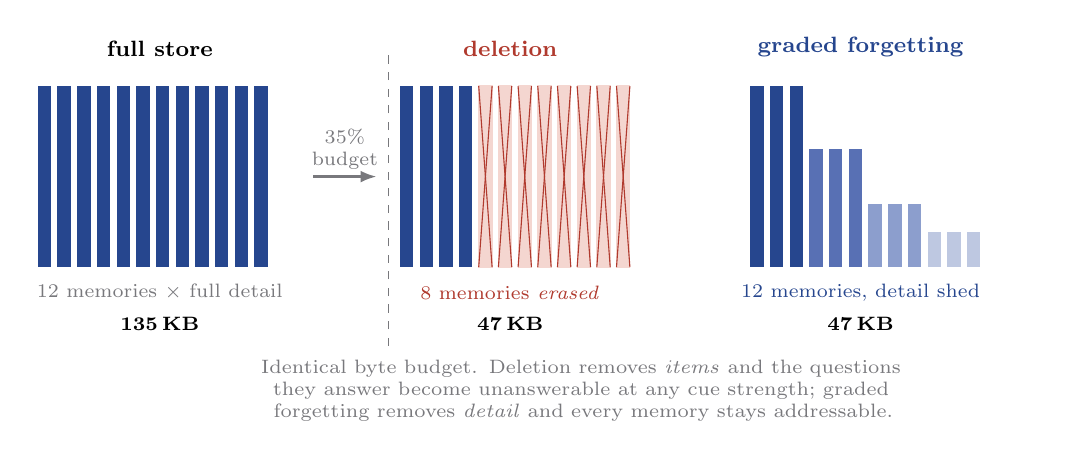
\begin{tikzpicture}[font=\small]
% -- full store
\node[anchor=south,font=\bfseries\footnotesize] at (1.55,2.55) {full store};
\foreach \i in {0,...,11}{
  \fill[keep] ({\i*0.25},0) rectangle ({\i*0.25+0.17},2.3);}
\node[font=\scriptsize,neut] at (1.55,-0.32) {12 memories $\times$ full detail};
\node[font=\scriptsize\bfseries] at (1.55,-0.72) {135\,KB};

% -- arrow
\draw[-{Latex[length=2mm]},neut,thick] (3.5,1.15) -- (4.3,1.15);
\node[font=\scriptsize,neut,align=center] at (3.9,1.5) {35\%\\budget};

% -- deletion
\node[anchor=south,font=\bfseries\footnotesize,lose] at (6.0,2.55) {deletion};
\foreach \i in {0,...,3}{
  \fill[keep] ({4.6+\i*0.25},0) rectangle ({4.6+\i*0.25+0.17},2.3);}
\foreach \i in {4,...,11}{
  \draw[loseL,fill=loseL] ({4.6+\i*0.25},0) rectangle ({4.6+\i*0.25+0.17},2.3);
  \draw[lose,thin] ({4.6+\i*0.25},0) -- ({4.6+\i*0.25+0.17},2.3);
  \draw[lose,thin] ({4.6+\i*0.25+0.17},0) -- ({4.6+\i*0.25},2.3);}
\node[font=\scriptsize,lose] at (6.0,-0.32) {8 memories \emph{erased}};
\node[font=\scriptsize\bfseries] at (6.0,-0.72) {47\,KB};

% -- demotion
\node[anchor=south,font=\bfseries\footnotesize,keep] at (10.45,2.55) {graded forgetting};
\foreach \i/\h/\c in {0/2.3/keep,1/2.3/keep,2/2.3/keep,3/1.5/fade1,4/1.5/fade1,
                      5/1.5/fade1,6/0.8/fade2,7/0.8/fade2,8/0.8/fade2,
                      9/0.45/fade3,10/0.45/fade3,11/0.45/fade3}{
  \fill[\c] ({9.05+\i*0.25},0) rectangle ({9.05+\i*0.25+0.17},\h);}
\node[font=\scriptsize,keep] at (10.45,-0.32) {12 memories, detail shed};
\node[font=\scriptsize\bfseries] at (10.45,-0.72) {47\,KB};

\draw[neut,dashed,thin] (4.45,-1.0) -- (4.45,2.75);
\node[font=\scriptsize,neut,anchor=north,align=center,text width=11.5cm]
  at (6.9,-1.05) {Identical byte budget. Deletion removes \emph{items} and
  the questions they answer become unanswerable at any cue strength;
  graded forgetting removes \emph{detail} and every memory stays addressable.};
\end{tikzpicture}
\caption{The two ways to meet a capacity bound. Both shed $65\%$ of the store.
Only one of them can still be asked about the material it gave up.}
\label{fig:mechanism}
\end{figure}

% =====================================================================
\section{Background: what deployed memory does}
\label{sec:background}

\paragraph{Everything is tokens.} We inspected both major vendor SDKs. Neither
the Anthropic Messages API nor the OpenAI Responses API has a memory role,
field, or content type; retrieved memory reaches the model as ordinary tokens
in the context window. Anthropic mounts a filesystem the agent reads with file
tools, yielding tool-result blocks; OpenAI concatenates into the prompt. Any
``memory schema'' is a rendering convention honoured because models are trained
on such shapes. This bounds what any memory architecture can do: the only lever
is \emph{which text enters the window}, which is precisely what a retention
policy decides.

\paragraph{Deletion is the universal policy.} Anthropic caps stores and
recommends manual removal; version history exists but is reachable only through
a developer-facing management API and is retained 30 days. Mem0's reconciler
issues \texttt{DELETE} with no recovery path. We note an empirical observation
about Mem0 in Sec.~\ref{sec:negative}: on our corpus its reconciler fired
\emph{zero} times in 381 ingestions, because the conversation contains almost
no contradictions - the consolidation mechanism is real but workload-dependent.

\begin{table}[t]
\caption{Retention mechanisms in deployed systems. The lower block is
unaddressed.}
\label{tab:gap}\centering\small\setlength{\tabcolsep}{7pt}
\begin{tabular}{@{}lcccc@{}}
\toprule
\textbf{Mechanism} & \textbf{RAG} & \textbf{Mem0} & \textbf{Anthropic} & \textbf{Ours} \\
\midrule
Persistent store                 & - & \checkmark & \checkmark & \checkmark \\
Consolidation                    & - & \checkmark & \checkmark & \checkmark \\
Point-in-time recovery           & - & -        & \checkmark\,(30\,d, out-of-band) & \checkmark \\
\midrule
Automatic ageing                 & - & - & - & \checkmark \\
Graded accessibility             & - & - & - & \checkmark \\
Capacity met without deletion    & - & - & - & \checkmark \\
In-band recovery of evicted material & - & - & - & \checkmark \\
\bottomrule
\end{tabular}
\end{table}

% =====================================================================
\section{Method}
\label{sec:method}

\subsection{Stage, tier, and the capacity policy}

Each memory carries a retention stage advancing with time since last access,
\begin{equation}
k \;=\; \min\!\big(K,\ \lfloor \lambda \ln(1+\Delta t)\rfloor\big),
\qquad p_{\text{base}}(k)=\gamma^{k},
\qquad \tau=\min\{k:\gamma^{k}<\theta\},
\label{eq:stage}
\end{equation}
and a fidelity tier $\ell(k)$ that rises with it. Tier 0 holds the verbatim
episode; successive tiers discard episodic detail and retain the routing
scaffold - tag, gist, topic - longest. Given a byte budget $B$, the policy
raises tiers on the oldest material until the store fits. \textbf{No memory is
removed.}

Mapped onto Anthropic Memory Stores this requires no new primitive: stage is a
path prefix (\texttt{/s0/}\ldots\texttt{/s7/}), demotion is an ordinary
\texttt{memories.update} that rewrites path and content, and because every
update creates an immutable version, the pre-demotion text is preserved for
free. Listing by \texttt{path\_prefix} makes ``everything at stage $\le 3$'' a
server-side query, and the store's \texttt{instructions} field steers read
order.

\subsection{Admission: a disjunction, not a product}

Retrieval admits a memory when
\begin{equation}
\underbrace{\sigma\!\cdot\!\gamma^{k}\ \ge\ \theta}_{\text{default traversal}}
\qquad\textbf{or}\qquad
\underbrace{\sigma\ \ge\ \theta_{\text{strong}}}_{\text{cued override}},
\qquad
\sigma=\exp\!\Big(\!-\tfrac{\lVert s_r-s^{*}\rVert^{2}}{2\delta_k^{2}}\Big),\
\delta_k=\delta_0(1+\eta k).
\label{eq:gate}
\end{equation}
Here $s^{*}$ is a contextual signal vector recorded at write time and $\delta_k$
widens with stage, so an aged trace is matched loosely by a gist-level cue.

The disjunction is essential and replaces a product form we originally
specified. Under $\sigma\cdot\gamma^{k}\ge\theta$ alone, a stage-7 memory
($\gamma^{k}=0.035$) requires $\sigma>1.42$ to be admitted, which is impossible
since $\sigma\le1$: old traces were unreachable at \emph{any} cue strength,
contradicting the model's own claim of recovery past $\tau$. Sec.~\ref{sec:negative}
reports the measured effect of this defect and its repair.


\begin{figure}[t]
\centering
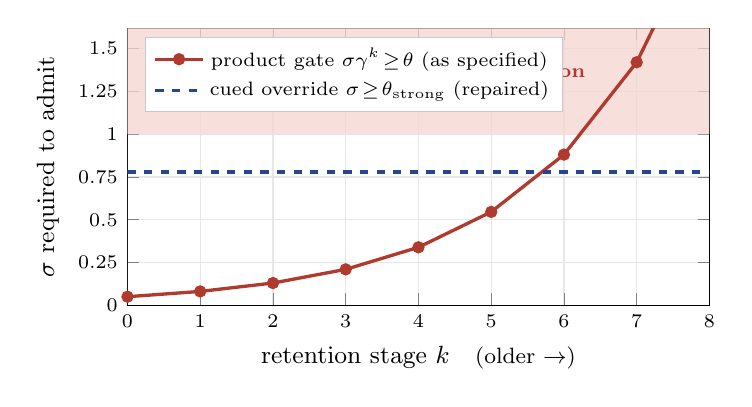
\begin{tikzpicture}
\begin{axis}[
  width=0.74\linewidth, height=5.1cm,
  xlabel={retention stage $k$ \ \ \footnotesize(older $\rightarrow$)},
  ylabel={$\sigma$ required to admit},
  xmin=0, xmax=8, ymin=0, ymax=1.62,
  xtick={0,1,2,3,4,5,6,7,8}, ytick={0,0.25,0.5,0.75,1.0,1.25,1.5},
  legend style={font=\scriptsize,at={(0.03,0.97)},anchor=north west,draw=neut!40},
  label style={font=\small}, tick label style={font=\scriptsize},
  grid=both, grid style={neut!18},
]
% impossible region
\addplot[draw=none,fill=loseL,opacity=.75,forget plot]
  coordinates {(0,1.0)(8,1.0)(8,1.62)(0,1.62)} \closedcycle;
\node[font=\scriptsize\bfseries,lose] at (axis cs:4,1.36) {impossible: $\sigma \le 1$ by definition};
\addplot[lose,very thick,mark=*,mark size=1.6pt]
  coordinates {(0,0.05)(1,0.081)(2,0.130)(3,0.210)(4,0.339)(5,0.546)(6,0.881)(7,1.421)(8,2.292)};
\addlegendentry{product gate $\sigma\gamma^{k}\!\ge\!\theta$ (as specified)}
\addplot[keep,very thick,dashed] coordinates {(0,0.78)(8,0.78)};
\addlegendentry{cued override $\sigma\!\ge\!\theta_{\text{strong}}$ (repaired)}
\end{axis}
\end{tikzpicture}
\caption{The admission rule forbade the recovery it was designed to provide.
Under the product form, a stage-7 memory needs $\sigma>1.42$ to be retrieved,
which no cue can supply. The disjunction of Eq.~\eqref{eq:gate} adds a flat
override, so a sufficiently specific cue reaches an aged trace while weak cues
still reach only recent ones.}
\label{fig:gate}
\end{figure}

% =====================================================================
\section{Recall-after-eviction}
\label{sec:protocol}

\paragraph{Why the obvious protocol fails.} The natural test - sample
questions, bucket by evidence age, compare under a budget - is uninformative,
and we report this because it cost us several experiments. Distillation writes
each dialogue turn into a median of \textbf{8} memories (mean $10.2$, max $43$);
\emph{no} question in our corpus depends on a single memory. Uniform random
eviction of $65\%$ of the store therefore destroys all copies of a question's
evidence with probability $0.65^{8}\approx0.03$, and we measured exactly that:
$8$ of $382$ questions. A random-eviction control matched the uncapped ceiling
not because uniform thinning preserves recall, but because it had destroyed
almost nothing.


\begin{figure}[t]
\centering
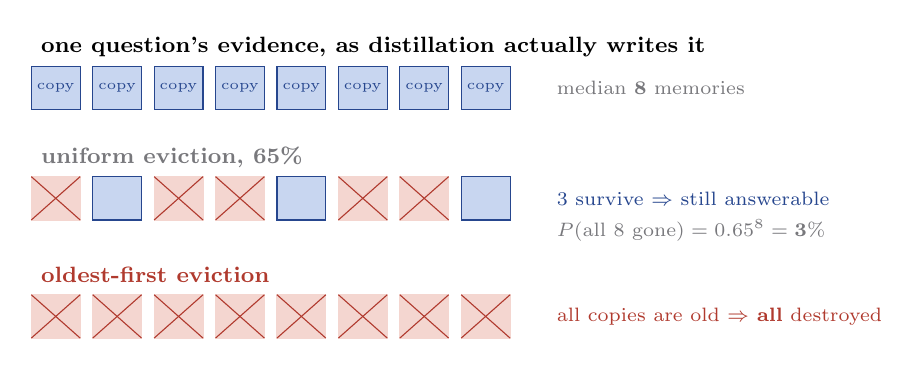
\begin{tikzpicture}[font=\small]
% evidence duplicated across 8 memories
\node[font=\bfseries\footnotesize,anchor=west] at (0,3.15)
  {one question's evidence, as distillation actually writes it};
\foreach \i in {0,...,7}{
  \fill[keepL,draw=keep] ({\i*0.78},2.35) rectangle ({\i*0.78+0.62},2.9);
  \node[font=\tiny,keep] at ({\i*0.78+0.31},2.63) {copy};}
\node[font=\scriptsize,neut,anchor=west] at (6.55,2.63) {median \textbf{8} memories};

% random eviction
\node[font=\footnotesize\bfseries,anchor=west,neut] at (0,1.75) {uniform eviction, 65\%};
\foreach \i/\k in {0/1,1/0,2/1,3/1,4/0,5/1,6/1,7/0}{
  \ifnum\k=1
    \draw[loseL,fill=loseL] ({\i*0.78},0.95) rectangle ({\i*0.78+0.62},1.5);
    \draw[lose,thin] ({\i*0.78},0.95) -- ({\i*0.78+0.62},1.5);
    \draw[lose,thin] ({\i*0.78+0.62},0.95) -- ({\i*0.78},1.5);
  \else
    \fill[keepL,draw=keep] ({\i*0.78},0.95) rectangle ({\i*0.78+0.62},1.5);
  \fi}
\node[font=\scriptsize,keep,anchor=west] at (6.55,1.22)
  {3 survive $\Rightarrow$ still answerable};
\node[font=\scriptsize,neut,anchor=west] at (6.55,0.82)
  {$P(\text{all }8\text{ gone})=0.65^{8}=\mathbf{3\%}$};

% oldest-first
\node[font=\footnotesize\bfseries,anchor=west,lose] at (0,0.25) {oldest-first eviction};
\foreach \i in {0,...,7}{
  \draw[loseL,fill=loseL] ({\i*0.78},-0.55) rectangle ({\i*0.78+0.62},0);
  \draw[lose,thin] ({\i*0.78},-0.55) -- ({\i*0.78+0.62},0);
  \draw[lose,thin] ({\i*0.78+0.62},-0.55) -- ({\i*0.78},0);}
\node[font=\scriptsize,lose,anchor=west] at (6.55,-0.28)
  {all copies are old $\Rightarrow$ \textbf{all} destroyed};
\end{tikzpicture}
\caption{Why stratifying random questions by age measures nothing. Evidence is
duplicated across a median of eight memories, so uniform eviction almost never
destroys a question's support; recency-ordered eviction removes a contiguous
block of time and takes every copy at once. A protocol must condition on
evidence actually having been erased.}
\label{fig:redundancy}
\end{figure}

\paragraph{The protocol.} Condition on the capability. Build one long timeline,
impose a byte budget $B$, and for each question determine whether the memories
carrying its gold evidence survived. Evaluate only the questions whose evidence
a destructive policy \emph{erased}, asking every system the same set:

\begin{center}\small
\begin{tabular}{@{}ll@{}}
\textbf{full} & evidence intact - the ceiling \\
\textbf{delete} & evidence removed outright - nothing to retrieve \\
\textbf{graded} & evidence demoted and compressed - faint but present \\
\end{tabular}
\end{center}

The claim reduces to one falsifiable question: does a compressed gist retain
enough to answer where a deleted memory retains nothing? A deletion policy
cannot score here regardless of retrieval quality, which is the point: the
protocol measures a capability rather than ranking retrievers.

% =====================================================================
\section{Results}
\label{sec:main}

\paragraph{Setup.} Three LoCoMo \citep{maharana2024locomo} conversations
concatenated into one 833-day timeline of 1{,}115 memories
($135{,}243$ bytes), budget $B=35\%$. Backbone Claude-Sonnet-4.5; judge
Claude-Haiku-4.5. Under \emph{delete-oldest}, $248$ of $382$ questions lose
their evidence entirely; their supporting turns have median age $675$ days
(range $200$--$833$) against $74$ days for the survivors, so the evicted set
is precisely the distant past. We sample $40$.

\begin{table}[t]
\caption{Recall of the evicted past. Same byte budget; same questions; the
policies differ only in how they meet it.}
\label{tab:main}\centering\small\setlength{\tabcolsep}{10pt}
\begin{tabular}{@{}lccl@{}}
\toprule
\textbf{Policy} & \textbf{Accuracy} & \textbf{Tokens/q} & \textbf{State of the evidence} \\
\midrule
full (uncapped)      & 75.0\% & 3,117 & intact - ceiling \\
delete-oldest        & \textcolor{bad}{\textbf{2.5\%}} & 2,806 & removed outright \\
\rowcolor{hl}
graded forgetting    & \textbf{60.0\%} & 33,423 & compressed to gist (mean tier $2.0$) \\
\bottomrule
\end{tabular}
\end{table}

Graded forgetting answers $60.0\%$ of questions about material that deletion
destroyed, recovering $80\%$ of the uncapped ceiling from tier-2 gists while
shedding the same $65\%$ of bytes. Deletion's $2.5\%$ is a single question
answered from incidental surviving context. The gap is $24\times$ and is not a
margin: no retrieval improvement can raise the deletion arm, because the
evidence is gone.

\paragraph{The cost.} Graded forgetting spends $33{,}423$ tokens per query
against $2{,}806$. This is an implementation artefact - our reconstruction
loop re-serialises the full accumulated evidence set each turn over a
1{,}115-memory graph - not a property of compression, but it is severe and
unresolved, and we return to it in Sec.~\ref{sec:limits}.

% =====================================================================
\section{Negative results, defects, and the noise floor}
\label{sec:negative}

We report these at length because they bound what the positive result means.

\paragraph{Graded forgetting does not improve retrieval.} Without capacity
pressure it ranks last or near-last in every setting we measured
(Table~\ref{tab:neg}). Compression costs accuracy whenever the store is small
enough that nothing needs forgetting.

\begin{table}[t]
\caption{Settings without capacity pressure. Graded forgetting is never best.}
\label{tab:neg}\centering\small\setlength{\tabcolsep}{7pt}
\begin{tabular}{@{}llccc@{}}
\toprule
\textbf{Setting} & \textbf{Backbone} & \textbf{Flat retrieval} & \textbf{Active recon.} & \textbf{Graded} \\
\midrule
LoCoMo, $n{=}90$            & gpt-5.6-luna      & \textbf{53.3} & 47.8 & 38.9 \\
LoCoMo, $n{=}90$            & claude-sonnet-4.5 & \textbf{57.8} & 48.9 & 34.4 \\
Memory Stores, flat layout  & claude-sonnet-4.5 & \textbf{58.3} & - & - \\
Memory Stores, staged tree  & claude-sonnet-4.5 & - & - & 58.3 \\
Memory Stores, query engine & claude-sonnet-4.5 & - & - & 50.0 \\
Mem0 (third-party)          & claude-sonnet-4.5 & \textbf{66.7} & - & - \\
\bottomrule
\end{tabular}
\end{table}

\paragraph{Three defects found only by execution.} (i) \emph{$\tau$ was
unreachable}: at our published $\gamma=0.72,\theta=0.05,K=8$, leaving the
working set requires $k>9.12$ while $K$ caps $k$ at $8$, so no trace could ever
be demoted and the efficiency mechanism never fired. (ii) \emph{The gate
forbade its own claim}: the product form of Eq.~\eqref{eq:gate} made old traces
unreachable at any $\sigma$; replacing it with the disjunction moved overall
accuracy $34.4\to50.0$ and flattened the age profile from
$100/33/25$ to $50/56/38$ across recent/mid/old buckets. (iii) \emph{A dead
rung}: tier 1 truncated at the first sentence break, a no-op on
single-sentence memories, making tier $1\!\to\!2$ a $211\!\to\!35$ character
cliff rather than a ladder.

\paragraph{A data defect that dominated everything.} Our distillation stored
timestamps as metadata and rendered them to the agent as day-offsets against an
unseen epoch: \textbf{1 of 367} memories contained an absolute date in its text,
against $46\%$ for Mem0. Temporal questions are $19$ of $90$ in LoCoMo and we
scored $0.0$--$4.3\%$ on them. Instructing the extractor to resolve relative
references against the session date raised coverage to $52$--$59\%$ and moved
temporal accuracy to $50.0\%$ (flat), $50.0\%$ (active) and $37.5\%$ (graded).
\textbf{One line of prompt moved the metric further than every retrieval
mechanism in this study combined}, which we take as evidence that memory-system
comparisons are currently dominated by extraction quality rather than
architecture.

\paragraph{Noise floor.} At $n{=}12$, one question is $8.3$ points; three
identical repeats of one configuration returned $66.7\%$ and a fourth returned
$58.3\%$. No comparison at that scale resolves less than roughly two questions,
and we do not draw conclusions from such gaps.

\paragraph{Attribution.} Ablating the store confirms the questions require it:
closed-book $8.9\%$, wrong-conversation memory $7.8\%$, correct memory $50.0\%$
- so $82\%$ of performance is memory-attributable, with multi-hop and temporal
at \emph{zero} closed-book. Open-domain is the exception ($17\%$ closed-book,
$33\%$ with wrong memory) and measures persona inference rather than recall.

% =====================================================================
\section{Limitations}
\label{sec:limits}

\textbf{A weak deletion baseline.} \emph{delete-oldest} is recency-ordered and
unsophisticated. An importance-scored or LLM-judged policy would retain more of
what matters, and the honest statement of our result is that compression beats
\emph{recency-ordered} deletion. We consider a learned eviction baseline the
most important missing comparison.

\textbf{One budget, one corpus, $n{=}40$.} The effect is large ($57.5$ points)
and will not vanish on resampling, but its shape across budgets is unmeasured;
a sweep is the obvious next experiment.

\textbf{Token cost.} $12\times$ the deletion arm, from an implementation that
re-sends accumulated evidence each turn. Deployment requires fixing this.

\textbf{Confabulation.} Reconstruction from a tier-$\ell$ memory is generative.
We attach provenance tiers to every reconstructed span and treat $\tau$ as the
boundary between \emph{recalled} and \emph{inferred}, but we have no
calibration benchmark and regard one as a prerequisite for deployment.

\textbf{Security.} Retrieval-induced consolidation amplifies prompt injection:
an injected memory that is retrieved is \emph{promoted}, so content crafted to
match frequent queries resists decay while legitimate memories sink past it.
The platform documentation raises the underlying threat; our mechanism worsens
it. Mitigations (consolidate only trusted-provenance writes; cap cumulative
promotion; separate stores by trust level) are proposed but unevaluated.

% =====================================================================
\section{Related work}

\paragraph{Memory systems for LLM agents.} Early persistent stores summarise
dialogue into a vector index \citep{zhong2024memorybank,langmem2025}.
Structured successors organise memory explicitly: A-Mem links LLM-authored
notes into a graph \citep{xu2025amem}; Zep maintains a bi-temporal knowledge
graph that invalidates outdated edges \citep{rasmussen2025zep}; AriGraph learns
a knowledge-graph world model with episodic memory \citep{anokhin2024arigraph};
MemoryOS imposes a short/mid/long-term hierarchy \citep{kang2025memoryos};
SeCom segments memory at topically coherent boundaries \citep{pan2025secom};
LiCoMemory uses a lightweight hierarchical index with temporal-aware search
\citep{huang2025licomemory}; and LightMem targets construction efficiency
\citep{fang2025lightmem}. Mem0 maintains a compact fact store through
LLM-issued add/update/delete \citep{chhikara2025mem0}, and reflective memory
management adds prospective and retrospective revision
\citep{tan2025reflective}. All of these grow monotonically or prune
destructively; none demotes. Recent surveys map the design space
\citep{hu2025memorysurvey,gao2026selfevolving} and argue that long-term memory
remains a principal deficiency of deployed agents
\citep{hatalis2023memorymatters,hendrycks2025agi}.

\paragraph{Retrieval, and retrieval as reconstruction.} Retrieval-augmented
generation established one-shot similarity retrieval over an external store
\citep{lewis2020rag}, later extended to graph-structured corpora
\citep{han2025graphrag}. Agentic variants move retrieval inside the reasoning
loop, issuing queries on demand \citep{li2025searcho1} or learning to do so
with reinforcement \citep{jin2025searchr1}. Closest to our setting,
\citet{ji2026mragent} recast memory access as active, multi-step
reconstruction over a Cue--Tag--Content graph and prove active retrieval
strictly more expressive than passive; we adopt that formulation for our
reconstruction loop and treat its store as append-only, which is precisely the
assumption we relax.

\paragraph{Deployed memory, and its retention policy.} Anthropic's Memory
Stores expose a versioned document store mounted into an agent sandbox, capped
at 10{,}000 entries, with consolidation available as a separate \emph{Dreams}
job \citep{anthropic2026memory,anthropic2026dreams}. OpenAI's Agents SDK
persists transcripts and compacts them when they grow
\citep{openai2026sessions}, while ChatGPT synthesises user memory in a
background pass \citep{openai2026dreaming}. Each is a production system; each
meets capacity by deleting, compacting or rewriting, and none offers graded,
reversible demotion.

\paragraph{Benchmarks.} LoCoMo provides long multi-session dialogues with
annotated supporting evidence \citep{maharana2024locomo}; LongMemEval extends
the horizon and adds knowledge-update questions \citep{wu2025longmemeval}.
Both hold history at a fixed size. Recent analyses find full-context prompting
remains a strong baseline at LoCoMo's scale
\citep{simplebaseline2025,evallongterm2025}, which is consistent with our
observation that capacity pressure - not question difficulty - is the
regime where retention policy matters. Cross-paper comparison is further
complicated by unstandardised judging protocols \citep{mem0bench2026}, so we
compare only within our own harness.

\paragraph{Cognitive foundations.} The staged, cue-dependent view of forgetting
descends from Ebbinghaus's retention curves \citep{ebbinghaus1885} and the
distinction between storage and retrieval strength in the New Theory of Disuse
\citep{bjork1992}, with ACT-R supplying an activation-decay formalism
\citep{anderson1998actr}. Encoding specificity holds that retrieval succeeds to
the degree that cues reinstate the encoding context
\citep{tulving1983,godden1975}, which motivates our signal vector.
Reconstructive accounts from \citet{bartlett1932} to predictive coding
\citep{clark2013} treat recall as assembly rather than readout; the
neuroscience of retrieval describes cue-triggered reactivation of engrams
\citep{frankland2019retrieval,rugg2025cogneuro,rashid2016engrams}, with
episodic and semantic memory dissociable in the hippocampus
\citep{manns2003semantic} and recovery of apparently lost traces well
documented \citep{aggleton1999,proust1913}. Content-addressable and sparse
distributed memories established that stored patterns can be recovered from
partial keys \citep{hopfield1982,kanerva1988}, which is the computational
analogue of the cued override in Eq.~\eqref{eq:gate}.

% =====================================================================
\section{Conclusion}

Deployed agent memory meets capacity by deleting, irreversibly, without
knowledge of future queries. We showed that it need not: under a hard budget,
shedding detail rather than items preserves $60.0\%$ answerability on material
that deletion reduces to $2.5\%$, at identical storage cost. We also showed, in
six settings, that the same mechanism does not improve ordinary retrieval and
usually harms it.

We take the combination seriously rather than apologetically. It says the value
of graded forgetting is not in answering better but in \emph{still being able to
answer at all} once the store will not fit - and that benchmarks which hold
history at a fixed, comfortable size cannot see the difference. The costs are
paid on every query; the benefit appears only at capacity. Evaluating agent
memory on longer histories, rather than harder questions, is in our view the
change the field most needs.

% =====================================================================
% =====================================================================
\section*{Use of AI in this work}

Per the ICLR 2027 AI Policy for Authors, we disclose the following. A large
language model was used substantially throughout this project, in categories
the policy lists as requiring disclosure.

\textbf{Methodology and experiment design.} The model proposed the
recall-after-eviction protocol, identified that age-stratified eviction is
uninformative under evidence redundancy, and designed the eviction policies and
their controls.

\textbf{Implementation.} All experimental code - the memory lifecycle, the
retrieval agents, the benchmark harnesses, and the analysis scripts - was
written by the model under author direction.

\textbf{Interpretation of results.} The model performed the analyses reported
in Sections 5 and 6, including the diagnosis of the admission-gate defect, the
evidence-redundancy measurement, and the date-encoding finding.

\textbf{Writing.} The model drafted this manuscript, including its figures.

\textbf{Experimental subject.} Claude Sonnet 4.5 and GPT-5.6 were additionally
used as the agent backbones under evaluation, and Claude Haiku 4.5 as the
LLM judge; these are experimental apparatus rather than authoring assistance.

The authors take full responsibility for all content, including every claim,
number and citation. All quantitative results were produced by executing the
released code; all citations were verified to resolve to real publications.

\begin{thebibliography}{99}\small

\bibitem[Aggleton \& Brown(1999)]{aggleton1999} J.~P. Aggleton and M.~W. Brown.
Episodic memory, amnesia, and the hippocampal--anterior thalamic axis.
\emph{Behavioral and Brain Sciences}, 22(3):425--444, 1999.

\bibitem[Anderson \& Lebiere(1998)]{anderson1998actr} J.~R. Anderson and
C.~Lebiere. \emph{The Atomic Components of Thought}. Lawrence Erlbaum
Associates, 1998.

\bibitem[Anokhin et al.(2024)]{anokhin2024arigraph} P.~Anokhin, N.~Semenov,
A.~Sorokin, D.~Evseev, A.~Kravchenko, M.~Burtsev, and E.~Burnaev. AriGraph:
Learning knowledge graph world models with episodic memory for LLM agents.
\emph{arXiv:2407.04363}, 2024.

\bibitem[Anthropic(2026a)]{anthropic2026memory} Anthropic. Using agent memory
- Managed Agents documentation, 2026.
\url{https://platform.claude.com/docs/en/managed-agents/memory}.

\bibitem[Anthropic(2026b)]{anthropic2026dreams} Anthropic. Dreams: memory
consolidation for Managed Agents, 2026.
\url{https://platform.claude.com/docs/en/managed-agents/dreams}.

\bibitem[Bartlett(1932)]{bartlett1932} F.~C. Bartlett. \emph{Remembering: A
Study in Experimental and Social Psychology}. Cambridge University Press, 1932.

\bibitem[Bjork \& Bjork(1992)]{bjork1992} R.~A. Bjork and E.~L. Bjork. A new
theory of disuse and an old theory of stimulus fluctuation. In \emph{From
Learning Processes to Cognitive Processes}, volume~2, pp.\ 35--67. Lawrence
Erlbaum, 1992.

\bibitem[Chhikara et al.(2025)]{chhikara2025mem0} P.~Chhikara, D.~Khant,
S.~Aryan, T.~Singh, and D.~Yadav. Mem0: Building production-ready AI agents
with scalable long-term memory. \emph{arXiv:2504.19413}, 2025.

\bibitem[Clark(2013)]{clark2013} A.~Clark. Whatever next? Predictive brains,
situated agents, and the future of cognitive science. \emph{Behavioral and
Brain Sciences}, 36(3):181--204, 2013.

\bibitem[Ebbinghaus(1885)]{ebbinghaus1885} H.~Ebbinghaus. \emph{\"Uber das
Ged\"achtnis: Untersuchungen zur experimentellen Psychologie}. Duncker \&
Humblot, 1885.

\bibitem[Fang et al.(2025)]{fang2025lightmem} J.~Fang, X.~Deng, H.~Xu,
Z.~Jiang, Y.~Tang, Z.~Xu, S.~Deng, Y.~Yao, M.~Wang, S.~Qiao, H.~Chen, and
N.~Zhang. LightMem: Lightweight and efficient memory-augmented generation.
\emph{arXiv:2510.18866}, 2025.

\bibitem[Frankland \& Josselyn(2019)]{frankland2019retrieval} P.~W. Frankland
and S.~A. Josselyn. The neurobiological foundation of memory retrieval.
\emph{Nature Neuroscience}, 22(10):1576--1585, 2019.

\bibitem[Gao et al.(2026)]{gao2026selfevolving} H.~Gao et al. A survey of
self-evolving agents: What, when, how, and where to evolve on the path to
artificial super intelligence. \emph{Transactions on Machine Learning
Research}, 2026.

\bibitem[Godden \& Baddeley(1975)]{godden1975} D.~R. Godden and A.~D. Baddeley.
Context-dependent memory in two natural environments: On land and underwater.
\emph{British Journal of Psychology}, 66(3):325--331, 1975.

\bibitem[Han et al.(2025)]{han2025graphrag} H.~Han et al.
Retrieval-augmented generation with graphs (GraphRAG).
\emph{arXiv:2501.00309}, 2025.

\bibitem[Hatalis et al.(2023)]{hatalis2023memorymatters} K.~Hatalis,
D.~Christou, J.~Myers, S.~Jones, K.~Lambert, A.~Amos-Binks, Z.~Dannenhauer, and
D.~Dannenhauer. Memory matters: The need to improve long-term memory in
LLM-agents. In \emph{Proceedings of the AAAI Symposium Series}, volume~2,
pp.\ 277--280, 2023.

\bibitem[Hendrycks et al.(2025)]{hendrycks2025agi} D.~Hendrycks et al. A
definition of AGI. \emph{arXiv:2510.18212}, 2025.

\bibitem[Hopfield(1982)]{hopfield1982} J.~J. Hopfield. Neural networks and
physical systems with emergent collective computational abilities.
\emph{Proceedings of the National Academy of Sciences}, 79(8):2554--2558, 1982.

\bibitem[Hu et al.(2025)]{hu2025memorysurvey} Y.~Hu, S.~Liu, Y.~Yue, G.~Zhang,
B.~Liu, F.~Zhu, J.~Lin, H.~Guo, S.~Dou, and Z.~Xi. Memory in the age of AI
agents. \emph{arXiv:2512.13564}, 2025.

\bibitem[Huang et al.(2025)]{huang2025licomemory} Z.~Huang, Z.~Tian, Q.~Guo,
F.~Zhang, Y.~Zhou, D.~Jiang, and X.~Zhou. LiCoMemory: Lightweight and
cognitive agentic memory for efficient long-term reasoning.
\emph{arXiv:2511.01448}, 2025.

\bibitem[Ji et al.(2026)]{ji2026mragent} S.~Ji, Y.~Li, and B.~Hooi. Memory is
reconstructed, not retrieved: Graph memory for LLM agents. In
\emph{Proceedings of the 43rd International Conference on Machine Learning},
PMLR 306, 2026.

\bibitem[Jin et al.(2025)]{jin2025searchr1} B.~Jin, H.~Zeng, Z.~Yue, D.~Wang,
H.~Zamani, and J.~Han. Search-R1: Training LLMs to reason and leverage search
engines with reinforcement learning. \emph{arXiv:2503.09516}, 2025.

\bibitem[Kanerva(1988)]{kanerva1988} P.~Kanerva. \emph{Sparse Distributed
Memory}. MIT Press, 1988.

\bibitem[Kang et al.(2025)]{kang2025memoryos} J.~Kang, M.~Ji, Z.~Zhao, and
T.~Bai. Memory OS of AI agent. \emph{arXiv:2506.06326}, 2025.

\bibitem[LangChain(2025)]{langmem2025} LangChain. LangMem SDK for agent
long-term memory, 2025. \url{https://blog.langchain.com/langmem-sdk-launch/}.

\bibitem[Lewis et al.(2020)]{lewis2020rag} P.~Lewis, E.~Perez, A.~Piktus,
F.~Petroni, V.~Karpukhin, N.~Goyal, H.~K\"uttler, M.~Lewis, W.~Yih,
T.~Rockt\"aschel, S.~Riedel, and D.~Kiela. Retrieval-augmented generation for
knowledge-intensive NLP tasks. In \emph{Advances in Neural Information
Processing Systems 33}, 2020.

\bibitem[Li et al.(2025)]{li2025searcho1} X.~Li, G.~Dong, J.~Jin, Y.~Zhang,
Y.~Zhou, Y.~Zhu, P.~Zhang, and Z.~Dou. Search-o1: Agentic search-enhanced
large reasoning models. In \emph{EMNLP}, pp.\ 5420--5438, 2025.

\bibitem[Maharana et al.(2024)]{maharana2024locomo} A.~Maharana, D.~Lee,
S.~Tulyakov, M.~Bansal, F.~Barbieri, and Y.~Fang. Evaluating very long-term
conversational memory of LLM agents. In \emph{ACL}, pp.\ 13851--13870, 2024.

\bibitem[Manns et al.(2003)]{manns2003semantic} J.~R. Manns, R.~O. Hopkins, and
L.~R. Squire. Semantic memory and the human hippocampus. \emph{Neuron},
38(1):127--133, 2003.

\bibitem[Mem0(2026)]{mem0bench2026} Mem0. LoCoMo vs.\ LongMemEval vs.\ BEAM:
the 2026 AI memory benchmark guide, 2026.
\url{https://mem0.ai/blog/ai-memory-benchmarks-in-2026}.

\bibitem[OpenAI(2026a)]{openai2026sessions} OpenAI. Sessions - OpenAI Agents
SDK documentation, 2026.
\url{https://openai.github.io/openai-agents-python/sessions/}.

\bibitem[OpenAI(2026b)]{openai2026dreaming} OpenAI. Dreaming: better memory for
a more helpful ChatGPT, 2026.
\url{https://openai.com/index/chatgpt-memory-dreaming/}.

\bibitem[Pan et al.(2025)]{pan2025secom} Z.~Pan, Q.~Wu, H.~Jiang, X.~Luo,
H.~Cheng, D.~Li, Y.~Yang, C.-Y. Lin, H.~V. Zhao, and L.~Qiu. SeCom: On memory
construction and retrieval for personalized conversational agents. In
\emph{ICLR}, 2025.

\bibitem[Proust(1913)]{proust1913} M.~Proust. \emph{Du c\^ot\'e de chez Swann}.
Grasset, 1913.

\bibitem[Rashid et al.(2016)]{rashid2016engrams} A.~J. Rashid, C.~Yan,
V.~Mercaldo, H.-L. Hsiang, S.~Park, C.~J. Cole, A.~De~Cristofaro, J.~Yu,
C.~Ramakrishnan, and S.~Y. Lee. Competition between engrams influences fear
memory formation and recall. \emph{Science}, 353(6297):383--387, 2016.

\bibitem[Rasmussen et al.(2025)]{rasmussen2025zep} P.~Rasmussen, P.~Paliychuk,
T.~Beauvais, J.~Ryan, and D.~Chalef. Zep: A temporal knowledge graph
architecture for agent memory. \emph{arXiv:2501.13956}, 2025.

\bibitem[Rugg \& Renoult(2025)]{rugg2025cogneuro} M.~D. Rugg and L.~Renoult.
The cognitive neuroscience of memory representation. \emph{Neuroscience \&
Biobehavioral Reviews}, 155:105450, 2025.

\bibitem[Tan et al.(2025)]{tan2025reflective} Z.~Tan, J.~Yan, I.-H. Hsu,
R.~Han, Z.~Wang, L.~Le, Y.~Song, Y.~Chen, H.~Palangi, and G.~Lee. In prospect
and retrospect: Reflective memory management for long-term personalized
dialogue agents. In \emph{ACL}, pp.\ 8416--8439, 2025.

\bibitem[Tulving(1983)]{tulving1983} E.~Tulving. \emph{Elements of Episodic
Memory}. Oxford University Press, 1983.

\bibitem[Wang et al.(2025)]{simplebaseline2025} A simple yet strong baseline
for long-term conversational memory of LLM agents. \emph{arXiv:2511.17208},
2025.

\bibitem[Wu et al.(2025)]{wu2025longmemeval} D.~Wu, H.~Wang, W.~Yu, Y.~Zhang,
K.~Chang, and D.~Yu. LongMemEval: Benchmarking chat assistants on long-term
interactive memory. In \emph{ICLR}, 2025.

\bibitem[Xu et al.(2025)]{xu2025amem} W.~Xu, Z.~Liang, K.~Mei, H.~Gao, J.~Tan,
and Y.~Zhang. A-MEM: Agentic memory for LLM agents. \emph{arXiv:2502.12110},
2025.

\bibitem[Zhang et al.(2025)]{evallongterm2025} Evaluating long-term memory for
long-context question answering. \emph{arXiv:2510.23730}, 2025.

\bibitem[Zhong et al.(2024)]{zhong2024memorybank} W.~Zhong, L.~Guo, Q.~Gao,
H.~Ye, and Y.~Wang. MemoryBank: Enhancing large language models with long-term
memory. In \emph{AAAI}, pp.\ 19724--19731, 2024.

\end{thebibliography}

\end{document}
